\documentclass[dvipdfmx,12pt, uplatex]{jsarticle}
\usepackage{amsmath,amsthm,amssymb,amsfonts,fancyhdr, multicol}
\usepackage{graphicx}

\renewcommand{\thesection}{\S \arabic{section}}
%\renewcommand{\thesubsection}{\thesection.\arabic{subsection}}

\newcommand{\ds}{\displaystyle}

\DeclareMathOperator{\cosech}{cosech}
\DeclareMathOperator{\sech}{sech}
\DeclareMathOperator{\csch}{csch}

\pagestyle{fancy}

\begin{document}

\chead{双曲線関数について}
\rhead{}
\lhead{}


\section{双曲線関数}

以下の3つの関数は\textbf{双曲線関数}と呼ばれる.
\[
  \sinh x = \frac{e^{x} - e^{-x}}{2}, \quad
  \cosh x = \frac{e^{x} + e^{-x}}{2}, \quad
  \tanh x = \frac{\sinh x}{\cosh x}
\]
それぞれ,hyperbolic sine $x$, hyperbolic cosine $x$, hyperbolic
tangent $x$ と読む.三角関数 $\sin, \cos, \tan$ と似た記号を使うが,明
らかにそれらとは異なる関数である.$\sinh$ で1つの記号であり,$\sin
hx$ではなく $\sinh x$ である.全く異なる定義であるにもかかわらず,次節
以降で見るように三角関数たちと非常によく似た性質を持っている.

\section{双曲線関数の微分}
定義から直ちにわかることは次の導関数たちの関係である.なお,三角関数たち
と同様に $\left(\cosh x\right)^2$ を $\cosh^2 x$ と書
く.$\sinh$ と $\tanh$ に関しても同様である.
\[
  \left( \sinh x\right)' = \cosh x, \quad
  \left( \cosh x\right)' = \sinh x, \quad
  \left( \tanh x\right)' = \frac{1}{\cosh^2 x}
\]
$\sin$ と $\cos$ の関係に似ているが,符号の反転が起こらないのでより単純
で覚えやすい.各々の関数のグラフの概形を調べよう.先に見せておくが,
図\ref{graph}のようになる.
\begin{figure}[h]
  \begin{center}
    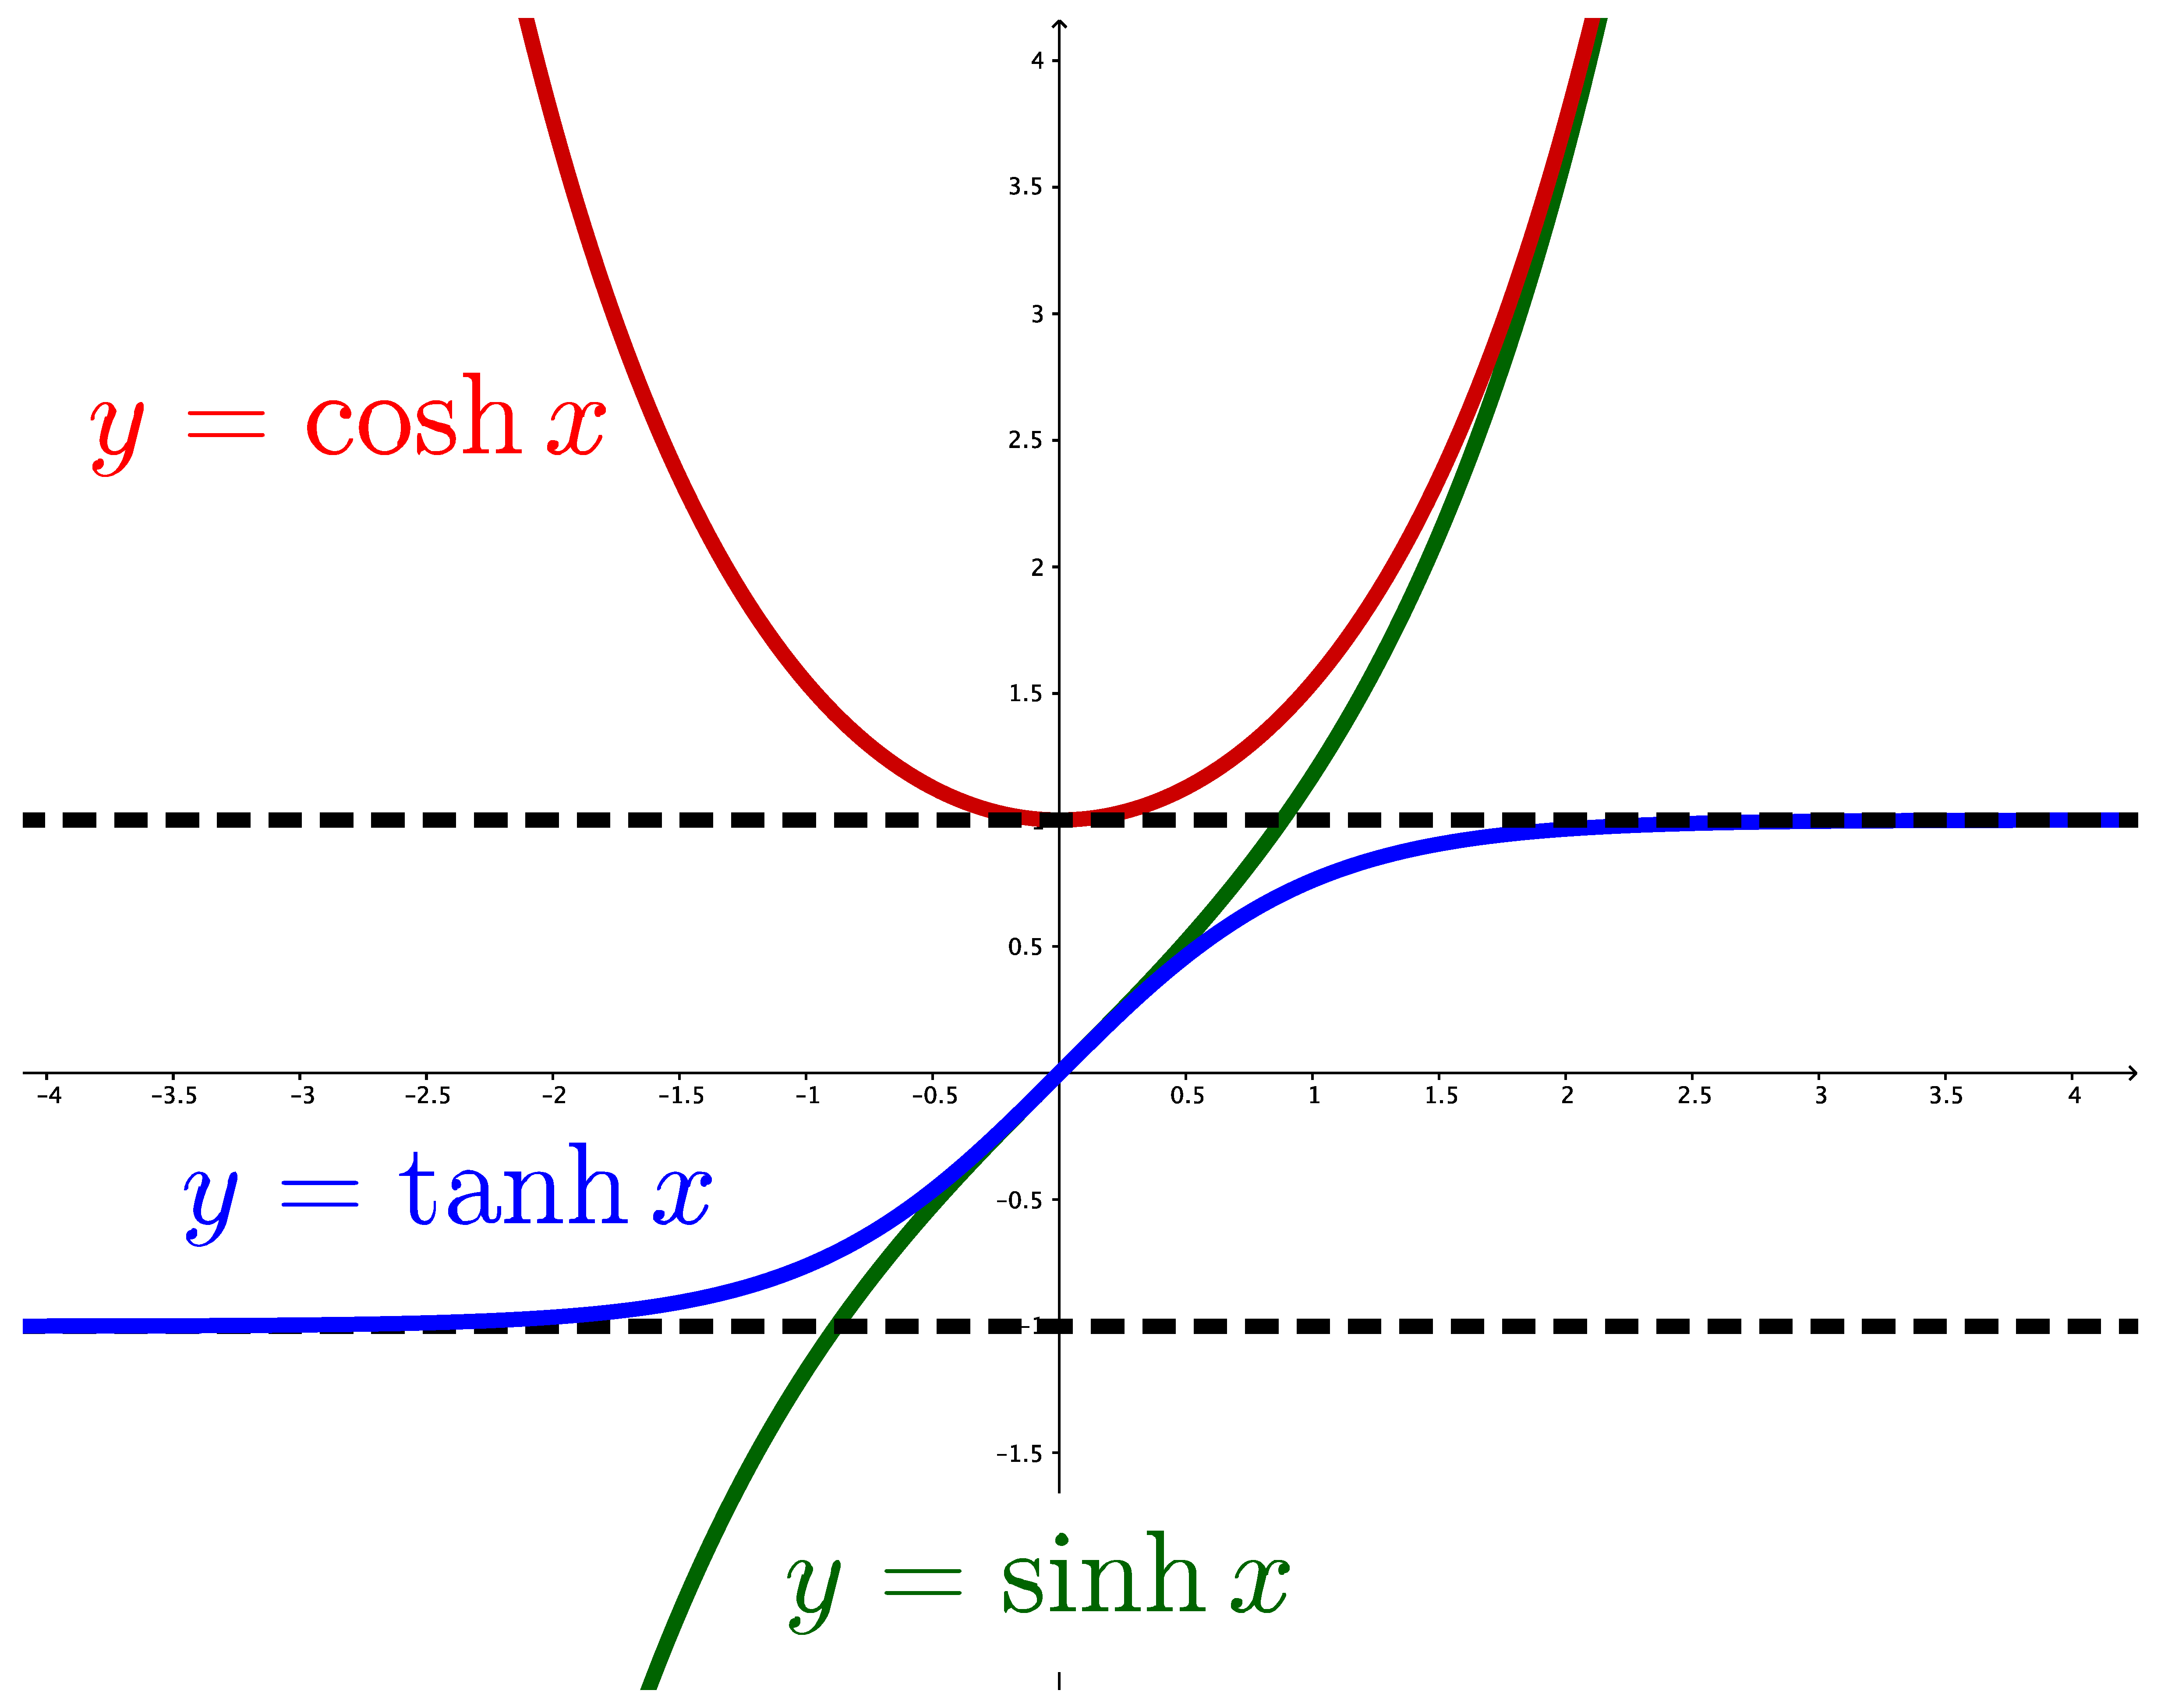
\includegraphics[width=7.7cm]{./pictures/graph.pdf}
    \caption{双曲線関数のグラフ}\label{graph}
  \end{center}
\end{figure}


では,$\sinh$ から調べていこう.$e^{x}, e^{-x}>0$ より
\[
  \left( \sinh x \right)'= \cosh x = \frac{e^{x} + e^{-x}}{2} >0
\]
がすぐにわかる.これより,$\sinh$ は $\mathbb{R}$ 上狭義単調増加
である.さらに,
\[
  \sinh 0 = \frac{e^0 - e^{0}}{2} = 0
\]
より,$\sinh x$ は $x=0$ を境に正負が入れ替わる.ま
た,$\sinh$ は $\mathbb{R}$ 上連続であり,
\[
  \lim_{x \to \infty} \sinh x = \infty, \quad  \lim_{x \to -\infty} \sinh x = -\infty
\]
であるから,$\sinh$ の値域は $(-\infty, \infty) \left( =
  \mathbb{R}\right)$ である.ついでに,
\[
\sinh (-x) = \frac{e^{-x} - e^{x}}{2} = -\frac{e^{x}-e^{-x}}{2} = -\sinh x
\]
より,$\sinh$ は奇関数であるから $y=\sinh x$ のグラフは原点対称である.
以上から,$y=\sinh x$ のグラフは図\ref{graph}の緑の曲線のようになること
がわかる.

次に,$\cosh$ について調べよう.$e^{x}, e^{-x}>0$ なので,
相加平均と相乗平均の関係から
\[
  \cosh x = \frac{e^{x} + e^{-x}}{2} \geq \sqrt{ e^{x} \cdot e^{-x}} = 1
\]
が成り立つ.等号が成立するのは $e^{x}=e^{-x}$ が成り立つとき,すなわ
ち,$x=0$ のときである.つまり,$\cosh x$ は $x=0$ のとき最小値 $1$ を
取ることがわかった.また,$\sinh$ の増減から
\[
  \left( \cosh x \right)' = \sinh x 
  \begin{cases}
    <0 & (x<0)\\
    =0 & (x=0)\\
    >0 & (x>0)
  \end{cases}
\]
より,$\cosh$ は $x \geq 0$ で狭義単調増加,$x \leq 0$ で狭義単調減少で
ある.さらに,$\cosh$ は $\mathbb{R}$ 上連続であり,
\[
\lim_{x \to \infty} \cosh x = \infty, \quad \lim_{x \to -\infty} \cosh x = \infty
\]
より,$\cosh$ の値域は $[1, \infty)$ である.ついでに,
\[
  \cosh (-x) = \frac{e^{-x} + e^{x}}{2} = \cosh x
\]
より,$\cosh$ は偶関数であるから $y=\cosh x$ のグラフは $y$ 軸について
対称である.以上から,$y=\cosh x$ のグラフは図\ref{graph}の赤の曲線のよ
うになることがわかる.

最後に,$\tanh$ について調べよう.
\[
  \left( \tanh x\right)' = \frac{1}{\cosh^2 x} >0
\]
より,$\tanh$ は $\mathbb{R}$ 上狭義単調増加である.なお,$\cosh x
\geq 1$ より $\cosh x \neq 0$ なので $\tanh$ は $\mathbb{R}$ の任意の点
において微分可能である.ここは記号が似ている $\tan$ とは事情が異なる.
さらに,
\[
  \tanh 0 = \frac{\sinh 0}{\cosh 0} = 0
\]
より,$\tanh x$ は $x=0$ を境に符号が入れ替わる.ま
た,$\tanh$ は $\mathbb{R}$ 上連続であり,
\begin{align*}
  \lim_{x \to \infty} \tanh x &= \lim_{x \to \infty} \frac{e^{x} - e^{-x}}{e^{x} + e^{-x}}
    = \lim_{x \to \infty} \frac{1 - e^{-2x}}{1 + e^{-2x}} = 1,\\
  \lim_{x \to -\infty} \tanh x &= \lim_{x \to -\infty} \frac{e^{x} -e^{-x}}{e^{x} + e^{-x}}
    =\lim_{x \to -\infty} \frac{e^{2x} -1}{e^{2x} +1} = -1
\end{align*}
より,$\tanh$ の値域は $(-1,1)$ である.ついでに,
\[
  \tanh (-x) = \frac{\sinh (-x)}{\cosh (-x)} = -\frac{\sinh x}{\cosh x} = -\tanh x
\]
より,$\tanh$ は奇関数であるから $y=\tanh x$ のグラフは原点対称である.
以上から,$y=\tanh x$ のグラフは図\ref{graph}の青の曲線のようになること
がわかる.


\section{双曲線関数の積分}

導関数の間の関係から $\sinh$ と $\cosh$ の不定積分についてもすぐに分か
る.なお,以後 $C$ は積分定数とする.
\[
\int \sinh x \ dx = \cosh x +C, \quad \int \cosh x \ dx = \sinh x +C
\]
こちらも三角関数のときと違って符号の反転は起こらない.また,三角関
数 $\tan$ を積分するのと全く同様の手法で $\tanh$ の不定積分も求められる.
つまり,
\[
  \int \tan x \ dx = \int \frac{\sin x}{\cos x} \ dx = \int
  -\frac{\left(\cos x\right)'}{\cos x} \ dx = -\log |\cos x | +C
\]
を真似て
\[
  \int \tanh x \ dx = \int \frac{\sinh x}{\cosh x} \ dx = \int
  \frac{\left( \cosh x \right)'}{\cosh x} \ dx = \log \left(\cosh x\right) +C
\]
を得る.なお,定義から $\cosh x >0$ なので$\log|\cosh x| =
\log\left(\cosh x\right)$ である.やはり三角関数のように符号の反転が起
こらないので最後にマイナスがつかない.このようにその定義式には指数関数
が含まれているにも関わらず,各々の微分や積分に関しては指数関数を表に出
すことなく導関数や不定積分を互いに表し合うことができる.そしてその相互
関係は三角関数たちのそれと非常によく似ている.

\section{双曲線関数の基本公式}
次に,双曲線関数の基本公式を紹介する.これらも三角関数とよく似ている.
\[
  \cosh^2 x - \sinh^2 x=1, \quad 1-\tanh^2 x = \frac{1}{\cosh^2 x}
\]
1つ目の等式は $\cosh, \sinh$ の定義式から容易に導ける.2つ目の式につい
ては1つ目の等式の両辺を $\cosh^2 x$ で割ればよい.ちなみに,三角関数では
\[
\cos^2 x + \sin^2 x = 1, \quad 1+\tan^2 x = \frac{1}{\cos^2 x}
\]
という関係式があったが,この2つ目の等式は先と同様に1つ目の等式の両辺
を $\cos^2 x$ で割って得られるであった.さて,既に紹介済みの $\tanh$ の
導関数は定義から容易に導くことができるのだが,ここで紹介した基本公式と
商の微分公式から
\[
  \left( \tanh x \right)' = \left( \frac{\sinh x}{\cosh x} \right)'
  =\frac{\cosh^2 x - \sinh^2 x}{\cosh^2 x} = \frac{1}{\cosh^2 x}
\]
と導くこともできる.これも以下の $\tan$ の導関数の導出過程と全く
同様である.
\[
  \left(\tan x\right)' = \left( \frac{\sin x}{\cos x}\right)' =
  \frac{\cos^2 x + \sin^2 x}{\cos^2 x} = \frac{1}{\cos^2 x}
\]
このように双曲線関数は三角関数とよく似た性質を持っているので,三角関数
と似たような方法で似たような公式を導くことができたりする.

\section{双曲線関数の加法定理}\label{addition}

三角関数の加法定理はよく知っているだろう.双曲線関数にも三角関数の
それと非常によく似た公式がある.それは以下の通りである.
\begin{align*}
  \sinh (x+y) &= (\sinh x) (\cosh y) + (\cosh x) (\sinh y)\\
  \sinh (x-y) &= (\sinh x) (\cosh y) - (\cosh x) (\sinh y)\\
  \cosh (x+y) &= (\cosh x) (\cosh y) + (\sinh x) (\sinh y)\\
  \cosh (x-y) &= (\cosh x) (\cosh y) - (\sinh x) (\sinh y)
\end{align*}
$\sinh$ を $\sin$ に,$\cosh$ を $\cos$ に置き換えれば上2つの等式は正に
三角関数 $\sin$ の加法定理そのものである.一方で,下2つの $\cosh$ に関
しては三角関数 $\cos$ の加法定理とは異なり符号の反転が起きないが,む
しろその分覚えやすく三角関数の加法定理よりも素直な公式であるとも言える.

三角関数の加法定理といえば,そこから派生する公式がたくさんあった.例え
ば,倍角の公式は以下のように $\sin$ と $\cos$ の加法定理からいとも簡単
に導出できるのであった.
\begin{align*}
  \sin 2x &= \sin(x+x)=(\sin x)(\cos x) + (\cos x)(\sin x) 
            = 2 (\sin x) (\cos x)\\
  \cos 2x &= \cos(x+x) = (\cos x)(\cos x) - (\sin x)(\sin x)
            =\cos^2 x - \sin^2 x
\end{align*}
さらに,
\[
  \cos^2 x + \sin^2 x = 1
\]
を用いると,$\cos$ の倍角の公式は以下のようにも書き換えられることも思い
出しておこう.
\[
\cos 2x = 1 - 2\sin^2 x = 2 \cos^2 x -1
\]
そして,この書き換えられた $\cos$ の倍角の公式を $\sin^2 x$ や $\cos^2
x$ について解き直すと以下の半角の公式が導けるのであった.
\[
  \sin^2 x = \frac{1-\cos 2x}{2}, \quad \cos^2 x = \frac{1+\cos 2x}{2}
\]

双曲線関数の加法定理を用いて上の三角関数の倍角の公式と半角の公式の導出
課程を真似ると,双曲線関数の倍角の公式と半角の公式に相当する等式が導け
る(双曲線関数の変数は角度ではないので「倍角」や「半角」といった用語は
適切ではないが,面倒なのでこう呼んでしまおう).すなわち,双曲線関数の
加法定理から倍角の公式
\begin{align*}
  \sinh 2x &= \sinh(x+x) = 2 (\sinh x)(\cosh x)\\
  \cosh 2x &= \cosh(x+x) = \cosh^2 x + \sinh^2 x
\end{align*}
が導かれる.さらに,双曲線関数の基本公式
\[
\cosh^2 x - \sinh^2 x=1
\]
を用いて $\cosh$ の倍角の公式は
\[
\cosh 2x = 1 + 2 \sinh^2 x = 2 \cosh^2 x -1
\]
と書き換えられる.そして,上の等式を $\sinh^2 x$ や $\cosh^2 x$ につい
て解き直して,以下の双曲線関数の半角の公式を得る.
\[
  \sinh^2 x = \frac{\cosh 2x -1}{2}, \quad \cosh^2 x = \frac{\cosh 2x +1}{2}
\]

三角関数にまつわる積分では基本公式や倍角・半角の公式を用いて式を書き換
えてることで計算を簡易化するという手法が有効であったように,双曲線関数
にまつわる積分に関してもこれらの基本公式や倍角・半角の公式は有用である.
例えば,$\sin^2$ や $\cos^2$ の不定積分は三角関数の半角の公式を用いて
\begin{align*}
  \int \sin^2 x \ dx &= \int \frac{1-\cos 2x}{2} \ dx 
                       = \frac{1}{2}x -\frac{1}{4} \sin 2x +C\\
  \int \cos^2 x \ dx &= \int \frac{1+\cos 2x}{2} \ dx
                       = \frac{1}{2}x + \frac{1}{4} \sin 2x +C
\end{align*}
と求められた.これを双曲線関数の場合に双曲線関数の半角の公式を用いて真似をすると
\begin{align*}
  \int \sinh^2 x \ dx &= \int \frac{\cosh 2x -1}{2} \ dx
                        = \frac{1}{4} \sinh 2x - \frac{1}{2} x +C\\
  \int \cosh^2 x \ dx &= \int \frac{\cosh 2x +1}{2} \ dx
                        =\frac{1}{4} \sinh 2x + \frac{1}{2} x +C
\end{align*}
を得る.同様に,$\sin^3, \cos^3, \sin^4, \cos^4, \ldots$ などの積分計算
に使われる手法をそのまま真似れば,$\sinh^3, \cosh^3, \sinh^4, \cosh^4,
\ldots$ などの不定積分も求められる.例えば,$\sinh^3$ なら
\[
\sinh^3 x = (\sinh^2 x ) \sinh x = (\cosh^2x-1) (\cosh x)'
\]
と書き換えられるので,$u=\cosh x$ とおく置換積分により
\[
  \int \sinh^3 x \ dx = \int \left( u^2-1 \right) \ du =
  \frac{1}{3}u^3-u +C = \frac{1}{3} \cosh^3 x - \cosh x +C
\]
を得る.また,例えば $\cosh^4$ であれば,
\begin{align*}
  \cosh^4 x &= \left( \cosh^2 x\right)^2 = \left( \frac{\cosh 2x
      +1}{2}\right)^2 = \frac{1}{4}\left( \cosh^2 2x + 2 \cosh 2x
    +1\right)\\
  &= \frac{1}{4} \left( \frac{ \cosh 4x +1}{2} + 2 \cos 2x +1\right)
    = \frac{1}{8} \cosh 4x + \frac{1}{2} \cosh 2x + \frac{3}{8}
\end{align*}
と変形できるので,
\[
  \int \cosh^4 x \ dx = \frac{1}{32} \sinh 4x + \frac{1}{4} \sinh 2x +
  \frac{3}{8}x +C
\]
を得る.このように,奇数乗か偶数乗によって計算の仕方が分かれるのも三角関
数の場合と同じである.さらに,$(\sinh^m x)(\cosh^n x)$ の積分
も $(\sin^m x)(\cos^n x)$ の積分と同じように $m,n$ の偶奇の組み合わせ
によって計算方法が分かれる.


\section{逆双曲線関数}

$\sinh$ は $\mathbb{R}$ 上狭義単調増加な関数であるから,その逆関
数 $\sinh^{-1}$ が存在する.同様に,$\tanh$ は $\mathbb{R}$ 上狭義単調
増加な関数であるからその逆関数 $\tanh^{-1}$ が存在する.

一方で,$\cosh$ は $\mathbb{R}$ 上で狭義単調増加でも狭義単調減少でもな
いので, $\cosh$ に逆関数は存在しない.しかしながら,$\cosh$ の定義域
を $[0, \infty)$ に制限した関数は狭義単調増加なので逆関数が存在する.こ
れを $\cosh^{-1}$ と書くことにする.

$\sinh^{-1}$ の定義域は $\sinh$ の値域,すなわち
$(-\infty, \infty) \; \left(= \mathbb{R}\right)$ であるか
ら,$\sinh^{-1}x$ と書いたとき $x$ は任意の実数を取り得る.一方
で,$\cosh^{-1}$ の定義域は $\cosh$ の値域,すなわち $[1, \infty)$ で
あり,$\tanh^{-1}$ の定義域は $\tanh$ の値域,すなわち  $(-1,1)$ であ
る.故に,$\cosh^{-1}x$ と書いたときは $x \geq 1$ が,$\tanh^{-1}x$ と
書いたとき $-1 < x < 1$ が自動的に仮定されていることに注意しよう.

ここで定義した $\sinh^{-1}, \, \cosh^{-1}, \tanh^{-1}$ をまとめ
て\textbf{逆双曲線関数}と呼ぶ.読み方はそれぞれ,hyperbolic sine
inverse, hyperbolic cosine invers, hyperbolic tangent invers である.逆
三角関数のときと同様に,ここでの $(-1)$ 乗は逆数を表す記号ではないこと
に注意しよう.

ちなみに,三角関数たちと同じように,各々の逆数として定義される関数には
以下のような記号が用意されている.
\[
\cosech x = \frac{1}{\sinh x}, \quad \sech x = \frac{1}{\cosh x}, \quad \coth x = \frac{1}{\tanh x}
\]
読み方はそれぞれ,hyperbolic cosecant, hyperbolic secant, hyperbolic
cotangent だろう,多分.$\cosech$ は長いので $\csch$
と書くこともあるらしい.


なお,ここでは $\cosh$ の定義域を $[0, \infty)$ に制限したが,もちろ
ん $(-\infty, 0]$ に制限した関数にも逆関数がある.$\cosh$ の定義域
を $[0, \infty)$ に制限した関数を $\cosh_{+}$ と書き,$(-\infty, 0]$ に
制限した関数を $\cosh_{-}$ と書くとすると,各々の逆関数の間に
は $\cosh_{-}^{-1} x = - \cosh_{+}^{-1}x$ という関係がある.上では(そ
してこれ以降も) $\cosh_{+}^{-1}$ を単に $\cosh^{-1}$ と書いている.

\section{逆双曲線関数の微分}\label{diff-inv}

前節で逆双曲線関数が定義できた.関数が定義されたらその導関数を調べたく
なるのは人として当然の欲求であろう.これに関しても逆三角関数の導関数を
求めるのと全く同様の手法が通用する.


$\sinh^{-1}$ の導関数を調べよう.$y=\sinh^{-1}x$ とおくと,$x=\sinh y$
である.逆関数の微分公式から

\[
  \left(\sinh^{-1} x\right)'= \frac{dy}{dx} = \frac{1}{\frac{dx}{dy}} = \frac{1}{\cosh y} =
  \frac{1}{\sqrt{1+\sinh^2 y}} = \frac{1}{\sqrt{1+x^2}}
\]
を得る.ここで,双曲線関数の基本公式から
\[
\cosh^2 y =1+ \sinh^2 y
\]
であり,$\cosh y>0$ より $\cosh y = \sqrt{1+\sinh^2 y}$ となることを用いた.

次に,$\cosh^{-1}$ の導関数を調べよう.$y=\cosh^{-1}x$ とおく
と,$x=\cosh y$ である.ただし,$\cosh^{-1}$ の定義から,$y \geq 0$ で
ある.逆関数の微分公式から
\[
  \left( \cosh^{-1}\right)' = \frac{dy}{dx} = \frac{1}{\frac{dx}{dy}}
  = \frac{1}{\sinh y} = \frac{1}{\sqrt{\cosh^2 y -1}} =
  \frac{1}{\sqrt{x^2-1}}
\]
を得る.ただし,$x>1$ であり,$x=1$ で $\cosh^{-1}x$ は微分不可能であ
る.ここで,双曲線関数の基本公式から
\[
\sinh^2 y = \cosh^2 y -1
\]
であり,$y > 0$ なので $\sinh y > 0$ より $\sinh y = \sqrt{\cosh^2
  y-1}$ となることを用いた.

最後に,$\tanh^{-1}$ の導関数を調べよう.$y=\tanh^{-1} x$ とおく
と,$x=\tanh y$ である.逆関数の微分公式から
\[
  \left( \tanh^{-1} x \right)' = \frac{dy}{dx} =
  \frac{1}{\frac{dx}{dy}} = \cosh^2 y = \frac{1}{1-\tanh^2 y} = \frac{1}{1-x^2}
\]
を得る.ここで,双曲線関数の基本公式
\[
1- \tanh^2 y = \frac{1}{\cosh^2 y}
\]
を用いた.

以上をまとめると,以下の通りである.
\[
\left( \sinh^{-1} x \right)' = \frac{1}{\sqrt{1+x^2}}, \quad 
\left( \cosh^{-1} x \right)' = \frac{1}{\sqrt{x^2-1}}, \quad
\left( \tanh^{-1} x \right)' = \frac{1}{1-x^2}
\]
逆三角関数の導関数の公式
\[
\left( \sin^{-1} x \right)' = \frac{1}{\sqrt{1-x^2}}, \quad
\left( \cos^{-1} x \right)' = -\frac{1}{\sqrt{1-x^2}}, \quad
\left( \tan^{-1} x \right)' = \frac{1}{1+x^2}
\]
と比べるとやはりよく似ている.導出方法はほぼ全く同じと言ってもよいだろ
う.似たような性質を持つものに似たような処理を施したのだから似たような
結果が出てくるのは当たり前といえば当たり前でもある.

\section{逆双曲線関数の積分}

微分の次は積分を調べたくなるのも人として当然の欲求である.逆双曲線関数
の不定積分を求める前に逆三角関数の積分を思い出そう.いずれ
も $f(x)$ を $1 \cdot f(x)$ と見なしての部分積分であった.
\begin{align*}
  & \int \sin^{-1} x \ dx = x \sin^{-1}x - \int \frac{x}{\sqrt{1-x^2}} \ dx 
    = x \sin^{-1} x + \sqrt{1-x^2} +C\\
  & \int \cos^{-1} x \ dx = x \cos^{-1} x + \int \frac{x}{\sqrt{1-x^2}} \ dx
    = x \cos^{-1} x - \sqrt{1-x^2} +C\\
  & \int \tan^{-1} x \ dx = x \tan^{-1} x - \int \frac{x}{1+x^2} \ dx
    = x \tan^{-1} x - \frac{1}{2} \log (1+x^2) +C
\end{align*}
逆双曲線関数の積分は上の計算をそっくりそのまま真似ればよい.
\begin{align*}
  & \int \sinh^{-1} x \ dx = x \sinh^{-1}x - \int \frac{x}{\sqrt{1+x^2}} \ dx
    = x \sinh^{-1} x - \sqrt{1+x^2} +C\\
  & \int \cosh^{-1} x \ dx = x \cosh^{-1}x - \int \frac{x}{\sqrt{x^2-1}} \ dx
    = x \cosh^{-1} x -\sqrt{x^2-1} +C\\
  & \int \tanh^{-1} x \ dx = x \tanh^{-1} x - \int \frac{x}{1-x^2} \ dx
    = x \tanh^{-1} x + \frac{1}{2} \log (1-x^2) +C
\end{align*}
くどいようだが,似たような性質を持つものに似たような処理を施したので,
やはり似たような結果が得られている.

\section{逆双曲線関数の明示式}\label{expl-inv}

逆双曲線関数の場合,$\sinh$ と $\tanh$ は定義域を制限することなく逆関数が
存在し,$\cosh$ に関しても定義域を $0$ 以上の実数に制限するだけなので,
逆三角関数の定義よりも易しい.しかも,逆三角関数と違って逆双曲線関数は
実は知っている関数を使って書き表すことができる.

$\sinh^{-1} x$ をよく知っている関数を使って表そう.逆関数の定義か
ら,$y=\sinh^{-1}x$ とは $x = \sinh y$ を $y$ について解いた式でもある.
つまり,$\sinh$ の定義式に立ち戻って
\[
  x= \frac{e^{y}-e^{-y}}{2}
\]
を $y$ について解けばよい.両辺を $2 e^y$ 倍して式を整理すると
\[
  \left( e^y\right)^2  - 2x \left( e^y\right) - 1 = 0
\]
を得る.2次方程式の解の公式より
\[
e^y = x \pm \sqrt{x^2+1}
\]
であるが,$e^y >0$ より,$e^y = x + \sqrt{x^2+1}$ であり,従って
\[
  y = \log \left( x + \sqrt{x^2+1} \right)
\]
を得る.これが $\sinh^{-1} x$ である.ここから単純な計算により $y'$ を求めることもできる.

次に,$\cosh^{-1}x$ をよく知っている関数を用いて表そう.といって
も,先と全く同様のことをするだけである.つまり,$x = \cosh
y$ を $y$ について解けばよい.ただし,$\cosh^{-1}$ の定義から,$ x \geq 1, \, y \geq
0$ である.先と同様に
\[
  x = \frac{e^{y} + e^{-y}}{2}
\]
を $e^y$ について解いて,
\[
  e^y = x \pm \sqrt{x^2-1}
\]
を得るが,$y\geq 0$ より,$e^y \geq 1$ であるから,$e^y = x + \sqrt{x^2-1}$ である.従って,
\[
  y = \log \left( x + \sqrt{x^2-1} \right) \quad \left( x \geq 1 \right)
\]
を得る.これが $\cosh^{-1} x$ である.この形から $y'$ を計算することも
できる.

最後に,$\tanh^{-1}x$ を知っている関数で書き表そう.つまり,
\[
x = \frac{e^{y}-e^{-y}}{e^{y}+e^{-y}}
\]
を $y$ について解けばよい.上式を整理して
\[
(1-x)e^{2y} = 1+x
\]
より,
\[
y = \frac{1}{2} \log \frac{1+x}{1-x}
\]
を得る.これが $\tanh^{-1}x$ である.やはり,この形から $y'$ を求めることもできる.

最後にまとめておくと,
\begin{align*}
&\sinh^{-1} x = \log \left( x+ \sqrt{x^2+1}\right)\\
&\cosh^{-1} x = \log \left( x+ \sqrt{x^2-1}\right) \; \; ( x \geq 1)\\
&\tanh^{-1} x = \frac{1}{2} \log \frac{1+x}{1-x} \; \; (-1 < x < 1)
\end{align*}
である.上の3つの式を逆双曲線関数の明示式と呼ぶことにする.

\section{逆双曲線関数にまつわる積分}

逆双曲線関数にまつわるいくつかの積分公式を紹介する.結果だけを覚えるよりも,
各々の公式の導出方法を漠然と覚えておくほうが応用が効く.むしろ結果だ
け覚える方が難しいのではないか.

\subsection{ $\ds \frac{1}{\sqrt{a^2+x^2}}$ の積分}\label{1a2x2}

\ref{diff-inv}, \ref{expl-inv}の結果から,
\[
 \int \frac{dx}{\sqrt{1+x^2}} \ dx = \sinh^{-1} x+C = \log \left( x+\sqrt{x^2+1}\right)+C
\]
を得る.これを用いて
\[
  \int \frac{dx}{\sqrt{a^2+x^2}} 
\]
を求めよう.ただし,$a>0$ とする.$u=\frac{x}{a}$ とおくと,$\frac{du}{dx}=\frac{1}{a}$ であるから
\[
  \int \frac{dx}{\sqrt{a^2+x^2}} = \int \frac{dx}{a \sqrt{1+\left(\frac{x}{a}\right)^2}}
  = \int \frac{du}{\sqrt{1+u^2}} = \sinh^{-1} u +C = \sinh^{-1} \frac{x}{a} +C
\]
を得る.当然ながら逆三角関数 $\sin^{-1}$ に関する以下の積分公式とよく似ている.
\[
 \int \frac{dx}{\sqrt{a^2-x^2}} \ dx = \sin^{-1}\frac{x}{a} +C \quad (a>0)
\]
さらに,$\sinh^{-1}$ の明示式から
\[
\int \frac{dx}{\sqrt{a^2+x^2}} = \log \left( \frac{x}{a} + \sqrt{\left(\frac{x}{a}\right)^2 +1} \right)+C
= \log \left( x + \sqrt{x^2 + a^2} \right) + C
\]
を得る.ただし,$C-\log a$ を改めて $C$ とおき直した.


\subsection{$\ds \sqrt{a^2+x^2}$ の積分}\label{a2x2}

$a>0$
とする.$\sqrt{a^2+x^2}$の不定積分を求めよう.$x=a \sinh u \left(
  \Leftrightarrow u= \sinh^{-1}\frac{x}{a}\right)$ とおく
と,$\frac{dx}{du}=a \cosh u$ より,
\begin{align*}
  \int \sqrt{a^2+x^2} \ dx &= \int \sqrt{a^2 + a^2 \sinh^2 u} \ \left( a \cosh u \right) \ du
  = a^2 \int \sqrt{1+\sinh^2u} \ \left( \cosh u\right) \ du\\
  &= a^2 \int \sqrt{\cosh^2u }\ \left( \cosh u \right) \ du = a^2 \int \cosh^2 u \ du\\
  &= a^2 \left( \frac{1}{2}u + \frac{1}{4} \sinh 2u\right) +C 
  = a^2 \left( \frac{1}{2}u + \frac{1}{2} \sinh u \cosh u\right)+C\\
  &= a^2 \left( \frac{1}{2} u + \frac{1}{2} \sinh u \sqrt{1+\sinh^2 u} \right) +C\\
  &= \frac{a^2}{2} \left( \sinh^{-1}\frac{x}{a} + \frac{x}{a} 
    \sqrt{1+\left( \frac{x}{a}\right)^2}\right) +C\\
  &= \frac{1}{2} \left( a^2 \sinh^{-1} \frac{x}{a} + x \sqrt{a^2 + x^2}\right) +C
\end{align*}
を得る.途中で双曲線関数の半角・倍角の公式(\ref{addition}参照)を用い
た.やはり,$\sin^{-1}$ に関する以下の積分公式によく似ている.これ
も $x=a \sin u$ とおいて全く同様に導出できる.
\[
  \int \sqrt{a^2-x^2} \ dx = \frac{1}{2} \left( a^2 \sin^{-1}\frac{x}{a} + x \sqrt{a^2-x^2}\right)+C
  \; (a>0)
\]
さらに,$\sinh^{-1}$ の明示式(\ref{expl-inv}参照)から
\[\tag{$\clubsuit$}
  \int \sqrt{a^2+x^2} \ dx 
  = \frac{1}{2}\left(a^2 \log \left( x+ \sqrt{a^2+x^2}\right) + x \sqrt{a^2+x^2}\right) +C
\]
を得る.ただし,$C-\frac{a^2}{2} \log a$ を改めて $C$ とおき直した.


\subsection{計算例}

さて,\S\ref{a2x2} で導出した公式 $(\clubsuit)$ はやや複雑であり,これ
を覚えるのは困難である.覚えにくい公式は結果を覚えるよりも,大まかな導
出方法を覚えておけばよい.つまり,「 $x=a \sinh u$ とおいて置換積分」と
いうことさえ覚えておけばよい.また,定積分の計算では必ずしも不定積分を
求めきる必要はない.例として,定積分
\[
  \int_{0}^{1} \sqrt{1+4x^2} \ dx
\]
を計算してみよう.
\[
\sqrt{1+4x^2} = 2\sqrt{\frac{1}{4} + x^2}
\]
より,これは公式 $(\clubsuit)$ で $a=\frac{1}{2}$ とおいた場合であ
る.$x=\frac{1}{2}\sinh u \left( \Leftrightarrow u =
  \sinh^{-1}2x\right) $ とおくと,$\frac{dx}{du} = \frac{1}{2} \cosh
u$ であり,積分範囲は
\[
\begin{array}{c|ccc}
  x & 0 & \to & 1\\ \hline
  u & 0 & \to & \alpha:=\sinh^{-1}2
\end{array}
\]
と変換される.$\sinh \alpha =2$ なので,種々の公式たちと合わせて
\[
  \begin{aligned}
    \int_{0}^{1} \sqrt{1+4x^2} \ dx &= \int_{0}^{\alpha} \sqrt{1+\sinh^2 u} 
    \left( \frac{1}{2} \cosh u \right) \ du = \frac{1}{2} \int_{0}^{\alpha} \cosh^2 u \ du\\
    &= \frac{1}{2} \left[ \frac{1}{2} u +\frac{1}{4} \sinh 2u \right]_{0}^{\alpha}
    =\frac{1}{4} \alpha + \frac{1}{8} \sinh \left(2\alpha\right) \\
    &= \frac{1}{4} \alpha + \frac{1}{4} \left(  \sinh \alpha \right)
    \left( \cosh \alpha \right) 
    = \frac{1}{4} \alpha + \frac{1}{4} \cdot 2 \ \sqrt{1+\sinh^2 \alpha}\\
    &= \frac{1}{4} \sinh^{-1}2 + \frac{\sqrt{5}}{2}
    = \frac{1}{4} \log\left(2+\sqrt{5}\right) + \frac{\sqrt{5}}{2}
\end{aligned}
\]
を得る.最後に,$\sinh^{-1}$ の明示式を用いたが,これを忘れてしまった場合は方程式
\[
  \alpha= \sinh^{-1}2 \; \Leftrightarrow \; 2 = \frac{e^{\alpha} - e^{-\alpha}}{2}
\]
を解けばよい.ちないみに,ここで求めた定積分の値は,放物
線 $y=x^2$ の $0 \leq x \leq 1$ の部分の長さに等しい.


\subsection{ $\ds \frac{1}{\sqrt{x^2-a^2}}$ の積分}

\ref{diff-inv}, \ref{expl-inv} の結果から,
\[
  \int \frac{dx}{x^2-1} = \cosh^{-1} x +C = \log \left( x+\sqrt{x^2-1} \right) +C \;\; (x >1)
\]
である.\S\ref{1a2x2}と同様に,これを用いて
\[
  \int \frac{dx}{\sqrt{x^2-a^2}} \; \; (x>a)
\]
を求めよう.ただし,$a>0$ とする.$u=\frac{x}{u}$ とおくと,$\frac{du}{dx}=\frac{1}{a}$ であるから,
\[
  \int \frac{dx}{\sqrt{x^2-a^2}} = \int \frac{dx}{a\sqrt{\left( \frac{x}{a}\right)^2-1}}
  = \int \frac{du}{\sqrt{u^2-1}} = \cosh^{-1} u +C = \cosh^{-1} \frac{x}{a} +C
\]
を得る.さらに,$\cosh^{-1}$ の明示式から
\[
  \int \frac{dx}{\sqrt{x^2-a^2}} = \log \left( \frac{x}{a} + \sqrt{\left( \frac{x}{a}\right)^2-1} \right)  +C
    = \log \left( x+ \sqrt{x^2-a^2} \right) +C
\]
を得る.ただし,$C-\log a$ を改めて $C$ とおき直した.

さて,上で求めた公式は $x>a>0$ においては正しいが,$x<-a<0$ においては
正しくない.従って,例えば以下のような定積分の計算にはそのままでは使えない.
\[
  \int_{-3}^{-2} \frac{dx}{\sqrt{x^2-1}}
\]
そこで,$x<-a<0$ のときも含む公式を求めよう.

$x<-a<0$ とする.$x=-t$ とおくと,$\frac{dx}{dt}=-1$ であり,$t > a > 0$ なので
\[
  \int \frac{dx}{\sqrt{x^2-a^2}} = -\int \frac{dt}{\sqrt{t^2-a^2}} = -\log\left( t + \sqrt{t^2-a^2}\right) +C
\]
を得る.ここで,
\[
  -\log \left( t + \sqrt{t^2-a^2} \right) = \log \frac{1}{t+\sqrt{t^2-a^2}} 
  = \log \left(t-\sqrt{t^2-a^2}\right) -\log a^2
\]
より,$C-\log a^2$ を改めて $C$ とおき直して
\[
  \int \frac{dx}{\sqrt{x^2-a^2}} = \log \left( -x -\sqrt{x^2-a^2}\right) +C
  =\log \left(-\left( x+\sqrt{x^2-a^2} \right)\right) +C
\]
を得る.これが $x<-a$ のときの公式である.

以上から,$x>a$ のときと $x<-a$ のときをまとめて以下の公式を得る.
\[
  \int \frac{dx}{\sqrt{x^2-a^2}} = \log \left| x+\sqrt{x^2-a^2} \right| +C \quad \left( \left|x \right| >a \right)
\]
これで積分区間が負の値を含む場合の定積分も容易に計算できる.ただ
し, $-a \leq x \leq a$ の範囲では関数が定義されていないので
\[
  \int_{-1}^{2} \frac{dx}{\sqrt{x^2-9}}
\]
などの定積分は定義されない.

\subsection{ $\ds \sqrt{x^2-a^2}$ の積分}

$a>0$ とする.$\sqrt{x^2-a^2}$ の不定積分を求めよう.

まずは,$x \geq a$
としておく.$u = \cosh^{-1}\frac{x}{a} \; \left( \Leftrightarrow x= a
  \cosh u\right)$ とおくと,$u \geq 0$ なので $\sinh u \geq 0$ であ
る. また,$\frac{dx}{du} = a \sinh u$ より

\begin{align*}
  \int \sqrt{x^2-a^2} \ dx &= \int \sqrt{a^2 - a^2 \cosh^2 u} \ \left( a \sinh u \right) \ du
  = a^2 \int \sqrt{1-\cosh^2 u} \; (\sinh u ) \ du\\
                           &= a^2 \int \sqrt{\sinh^2 u} \ (\sinh u ) \ du
                             = a^2 \int \sinh^2 u \ du\\
                           &= a^2 \left( -\frac{1}{2}u+\frac{1}{4} \sinh 2u\right)+C
                             =a^2\left( -\frac{1}{2} u + \frac{1}{2} \sinh u \cosh u\right) +C\\
                           &= a^2\left( -\frac{1}{2} u + \frac{1}{2} \sqrt{\cosh^2 u -1} \ \cosh u \right) +C\\
                           &=\frac{a^2}{2} \left( -\cosh^{-1} \frac{x}{a}  
                             + \frac{x}{a} \sqrt{\left(\frac{x}{a}\right)^2-1} \right) +C\\
                           &= \frac{1}{2} \left( -a^2 \cosh^{-1} \frac{x}{a} + x \sqrt{x^2-a^2}\right)+C
\end{align*}
を得る.途中で双曲線関数の半角・倍角の公式(\ref{addition}参照)を用い
た.さらに,$\cosh^{-1}$ の明示式(\ref{expl-inv}参照)から
\[
  \int \sqrt{x^2-a^2} \ dx=\frac{1}{2} \left( -a^2 \log \left( x+ \sqrt{x^2-a^2} \right)+ x\sqrt{x^2-a^2}\right)+C \;
  (x \geq a)
\]
を得る.ただし,$C-\frac{a^2}{2} \log a$ を改めて $C$ とおき直した.


次に,$x \leq -a$ とする.$x=-t$ とおくと,$\frac{dx}{dt} = -1$ であり,$t \geq a$ なので
\[
  \int \sqrt{x^2-a^2} \ dx = -\int \sqrt{t^2-a^2} \ dt = -\frac{1}{2} \left( -a^2 \log \left( t+\sqrt{t^2-a^2} \right)
    + t \sqrt{t^2-a^2} \right)+C
\]
を得る.ここで,
\[
  -\log\left( t+\sqrt{t^2-a^2}\right) = \log \frac{1}{t+\sqrt{t^2-a^2}} 
  = \log \left( t - \sqrt{ t^2-a^2}\right) - \log a^2
\]
より,$C-\frac{a^2}{2}\log a^2$ を改めて $C$ とおき直して以下を得る.
\[
  \int \sqrt{x^2-a^2} \ dx = \frac{1}{2}\left( -a^2 \log \left( -\left(x + \sqrt{x^2-a^2}\right)\right) 
        + x\sqrt{x^2-a^2}\right)+C \; (x \leq -a)
\]

以上から,$x \geq a$ のときと $x \leq -a$ のときをまとめて以下の公式を得る.
\[
  \int \sqrt{x^2-a^2} \ dx = \frac{1}{2} \left( -a^2 \log \left| x + \sqrt{x^2-a^2}\right| + x\sqrt{x^2-a^2}\right) +C
  \; \left( \left|x \right| \geq a \right)
\]
さらに,\S\ref{a2x2}の結果と合わせて以下の公式を得る.
\[
  \int \sqrt{x^2 +A} \ dx = \frac{1}{2} \left( x \sqrt{x^2 +A} + 
    A \log \left| x + \sqrt{ x^2 + A} \right| \right) +C
\]
$A=a^2>0$ のときが,\S\ref{a2x2}の公式で,$A=-a^2<0$ のときが,今節の公式である.

\subsection{ $\ds \frac{1}{a^2-x^2}$ の積分}

\ref{diff-inv}, \ref{expl-inv}の結果から,
\[
  \int \frac{dx}{1-x^2} = \tanh^{-1} x +C = \frac{1}{2} \log \frac{1+x}{1-x} \; (-1 < x < 1)
\]
を得る.これを用いて
\[
  \int \frac{dx}{a^2-x^2} \quad \left( -a < x < a\right)
\]
を求めよう.ただし,$a>0$ とする.$u=\frac{x}{u}$ とおくと,$\frac{du}{dx} = \frac{1}{a}$ であるから
\[
  \int \frac{dx}{a^2-x^2} = \frac{1}{a} \int \frac{du}{1-u^2}
  = \frac{1}{a} \tanh^{-1} u +C =\frac{1}{a} \tanh^{-1} \frac{x}{a} +C
\]
を得る.やはり逆三角関数 $\tan^{-1}$ に関する公式
\[
  \int \frac{dx}{a^2+x^2} = \frac{1}{a} \tan^{-1} \frac{x}{a} +C
\]
とよく似ている.さらに,$\tanh^{-1}$ の明示式から
\[
  \int \frac{dx}{a^2-x^2} = \frac{1}{2a} \log \frac{a+x}{a-x} \; \left( -a < x < a\right)
\]
を得る.

さて,$\tan^{-1}$ との類似性を見るためにあえて上のように導出したが,この積分は
\[
  \frac{1}{a^2-x^2} - \frac{1}{(a+x)(a-x)} = \frac{1}{2a} \left( \frac{1}{a+x} + \frac{1}{a-x}\right) 
\]
という部分分数分解を用いて
\[
  \int \frac{dx}{a^2-x^2} = \frac{1}{2a}\left( \log | a+x| - \log |a-x| \right) 
  = \frac{1}{2a} \log \left| \frac{a+x}{a-x} \right| +C
\]
と求める方が一般的である.しかもこれなら $ -a < x < a$ という制限はつかない.


\section{おまけ}

初めに三角関数と双曲線関数は全く異なる定義にも関わらずよく似た性質を持っ
ていると書いたが,実は複素関数(つまり,定義域や値域が複素数の範囲に広
がった関数)として見ると両者は定義もよく似ている.以下,$i$ を虚数単位
とする.オイラーの公式
\[
  e^{i x} = \cos x + i \sin x 
\]
の $x$ に $-x$ を代入すると,
\[
  e^{-i x} = \cos x - i \sin x
\]
を得る.上の2式を連立して $\sin x$ と $\cos x$ について解くと
\[
  \cos x = \frac{e^{ix} + e^{-ix}}{2}, \quad \sin x = \frac{e^{ix} - e^{-ix}}{2i}
\]
を得る.実はこれが複素関数としての $\cos$ と $\sin$ の定義である.この
形は双曲線関数
\[
\cosh x = \frac{e^{x} + e^{-x}}{2}, \quad \sinh x = \frac{e^{x} - e^{-x}}{2}
\]
とよく似ている.両者を見比べると
\[
\cos x = \cosh ix, \quad i \sin x = \sinh ix
\]
という関係が見て取れる.ついでに,
\[
  i\tan x = \tanh ix
\]
という関係もすぐに分かる.これらを見れば三角関数と双曲線関数が似
たような性質持っていること,さらには,所々で符号が入れ
変わるのも虚数単位の性質
\[
  i^2 = -1
\]
から納得できるだろう.

\newpage

\section{三角関数と双曲線関数の類似性}

三角関数・逆三角関数と双曲線関数・逆双曲線関数にまつわる積分についてま
とめておく.ただし,以下では表示を簡単にするため積分定数は省略してある.美しい.

\begin{table}[h]
  \renewcommand{\arraystretch}{2}
  \begin{center}
    \fontsize{9pt}{0pt}
    \begin{tabular}{l|l}
      \multicolumn{1}{c|}{三角関数・逆三角関数} & \multicolumn{1}{|c}{双曲線関数・逆双曲線関数} \\ \hline  
      $\ds \int \sin x \ dx = -\cos x$ & $\ds \int \sinh x \ dx = \cosh x$ \\
      $\ds \int \cos x \ dx = \sin x$ & $\ds \int \cosh x \ dx = \sinh x $ \\
      $\ds \int \tan x \ dx = -\log |\cos x|$ & $\ds \int \tanh x \ dx = \log ( \cosh x)$\\
      $\ds \int \sin^2 x \ dx = \frac{1}{2}x - \frac{1}{4}\sin 2x$ &
      $\ds \int \sinh^2 x \ dx = -\frac{1}{2}x + \frac{1}{4} \sinh 2x$\\
      $\ds \int \cos^2 x \ dx = \frac{1}{2}x + \frac{1}{4} \sin 2x$ &
      $\ds \int \cosh^2 x \ dx = \frac{1}{2}x + \frac{1}{4}\sinh 2x$\\
      $\ds \int \sin^{-1}x \ dx = x \sin^{-1} x + \sqrt{1-x^2}$ &
      $\ds \int \sinh^{-1} x \ dx = x \sinh^{-1} x - \sqrt{1+x^2}$\\
      $\ds \int \cos^{-1} x \ dx = x \cos^{-1} x - \sqrt{1-x^2}$ &
      $\ds \int \cosh^{-1} x \ dx = x \cosh^{-1} x - \sqrt{x^2-1}$\\
      $\ds \int \tan^{-1} x \ dx = x \tan^{-1} x -\log \sqrt{1+x^2}$ &
      $\ds \int \tanh^{-1} x \ dx = x \tanh^{-1} x + \log \sqrt{1-x^2}$\\
      $\ds \int \frac{dx}{\sqrt{1-x^2}} = \sin^{-1}x$ &
      $\ds \int \frac{dx}{\sqrt{1+x^2}} = \sinh^{-1}x$\\
      $\ds \int \frac{dx}{1+x^2} = \tan^{-1} x$ &
      $\ds \int \frac{dx}{1-x^2} = \tanh^{-1} x\;\; \left(|x| <1 \right)$\\ 
      $\ds \int \sqrt{1-x^2} \ dx =\frac{1}{2}\left( \sin^{-1} x + x \sqrt{1-x^2}\right)$ &
      $\ds \int \sqrt{1+x^2} \ dx = \frac{1}{2} \left( \sinh^{-1}x + x \sqrt{1+x^2}\right)$
    \end{tabular}
  \end{center}
\end{table}

\end{document}
